\documentclass[11pt]{article}
\usepackage{geometry}                % See geometry.pdf to learn the layout options. There are lots.
\geometry{a4paper}                   % ... or a4paper or a5paper or ... 
%\geometry{landscape}                % Activate for for rotated page geometry
%\usepackage[parfill]{parskip}    % Activate to begin paragraphs with an empty line rather than an indent
\usepackage{graphicx}
\usepackage{amssymb}
\usepackage{epstopdf}
\usepackage[german, english]{babel}
\usepackage[utf8]{inputenc}
\usepackage{hyperref}
\usepackage{multicol}
\usepackage[table]{xcolor}% http://ctan.org/pkg/xcolor

\DeclareGraphicsRule{.tif}{png}{.png}{`convert #1 `dirname #1`/`basename #1 .tif`.png}

\title{Humanoid Robotics @ HTL Leonding}
\author{Annual Report 2018 / 2019}
%\date{}                                           % Activate to display a given date or no date

\hyphenation{Le-on-ding}

\begin{document}
\begin{titlepage}
\begin{flushright}

\includegraphics[scale=.85]{../img/htlleondinglogo.png}\\
\end{flushright}

\vspace{2em}

\begin{center}
{\Huge Humanoid Robotics @ HTL Leonding} \\[2em]
\includegraphics[scale=0.55]{img/Titlepage.png}\\[2em]
{\LARGE Annual Report 2018 / 2019}
\end{center}
\end{titlepage}

\tableofcontents
\newpage

\section{Introduction}
This report lists the activities of the Humanoid Robotics Team at the HTL Leonding during the school year~2018/2019, i.e., from September 1, 2018 to June 30, 2019. There is a good number of activities we are proud of to mention here. We also want to be pretty clear that only  a very brief overview is given and many details are left out to keep the report short. If there are any further questions the team lead can be contacted via \\[1em]
Peter Bauer\\
HTL Leonding, Department of Informatics\\
Limesstraße 12 -- 14\\
4060 Leonding\\
Fon: +43 676 6173320\\
Mail: p.bauer@htl-leonding.ac.at

\section{About Humanoid Robotics @ HTL Leonding}
Humanoid Robotics @ HTL Leonding is an initiative to motivate students of the HTL Leonding to deal with autonomous systems in general and with humanoid robots in particular. Furthermore students shall gain first experience in working on a software project within a larger team which implies the usual parameters like communication issues between team members, significantly large code bases, need for documentation, thorough tests, etc. Finally strictly motivate our students to take part in different robot competitions offered by the RoboCup Organization to get a clear feedback how well our teams are doing their job.

Since the HTL Leonding has a clear focus on software and no expertise in mechanical engineering a robot platform called {\em Nao} which is a standard platform from Softbank Robotics is used. This platform includes a humanoid robot (as it can be seen on the title page), an operating system called NAOqi which is a Linux kernel augmented by a set of libraries to control the robot's hardware and a set of software tools to program the robot. The Naos can be programmed in a great number of different programming languages but a proprietary graphical environment (Choregraphe), Python, and  C++ is mainly used.

As it requires already a good knowledge in software development and its related tooling to handle the C++ development stack we do an introductory phase for second graders where Choregraphe can be used as a programming environment. Nevertheless the students shall take part in the Demo Humanoid Challenge of the RoboCup Junior Austrian Open where less complex programming tasks which can be mastered by freshmen are requested.

After this the students may chose to move into the so-called soccer team which prepares to take part in the Standard Platform League which is a soccer competition where only Naos are allowed to take part. Here the Naos have to act autonomously as soccer players where two teams of five Naos play a soccer game on a 9 x 6 m large field (see figure~\ref{fig:soccerField}). To program the robots it is necessary to work deeply in the fields of computer vision, strategy, planning, motion, etc. Therefore, only university level schools take part in this league and it is one of the big goals to take part as the first technical college being formally on pre-university level.

\begin{figure}
\begin{center}
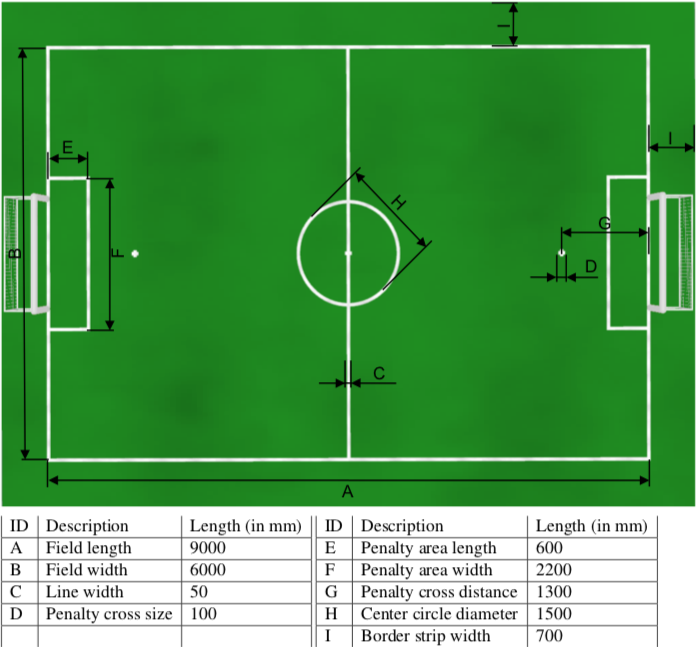
\includegraphics[scale=0.38]{img/soccerField.png}
%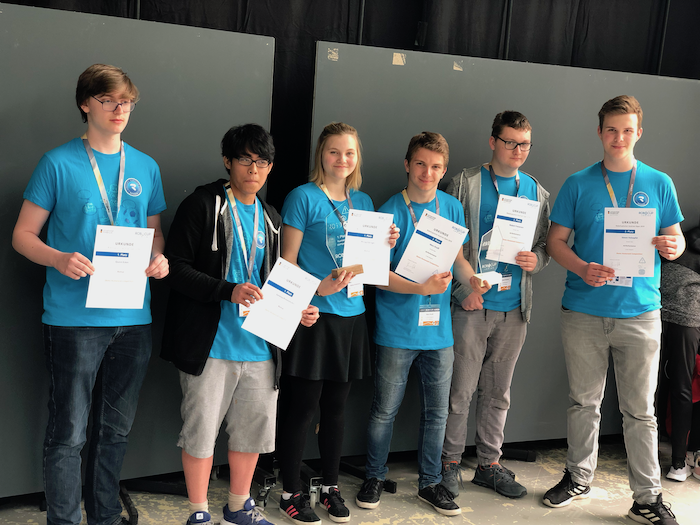
\includegraphics[scale=0.38]{img/rcjCeremony.png}
\end{center}
\caption{Dimensions of a Soccer 'Field at the Standard Platform League}
\label{fig:soccerField}
\end{figure}

\section{The Team}
Building a strong team of students and teachers who do a very focused work is an all time target we have in mind. Especially a smooth hand-over from one student generation to a next is a central topic. The more we are happy that we were able to increase the head count from six  to eighteen developers compared to the last period under report. The team members are the following: 

\begin{multicols}{2}
\begin{itemize}
	\item Erik Mayrhofer (4BHIF)
	\item Jan Neuburger (4BHIF)
	\item Florian Schwarcz (4BHIF)
	\item Max Wal (4BHIF)
	\item Lukas Gaisbauer (3BHIF)
	\item Florentin Gewessler (3BHIF)
	\item Christoph Knoll (3BHIF)
	\item Georg Sengstbratl (3BHIF)
	\item Jakob Wögerbauer (3BHIF)
	\item Nadia Bajim (2AHIF)
	\item Natalie Herzog (2AHIF)
	\item Emina Sljivic (2AHIF)
	\item Robert Freiseisen (2BHIF)
	\item Simon Holzapfel (2BHIF)
	\item Marc Kruiß (2BHIF)
	\item Quirin Ecker (2AHITM)
	\item Philipp Edlinger (2AHITM)
	\item Vanessa Primetzhofer (2AHITM)
\end{itemize}
\end{multicols}

Furthermore we took efforts to newly establish a promotion team which supports us to make our activities better visible to the public. The team members of the promotion team are

\begin{multicols}{2}
\begin{itemize}
	\item Samuel Kowatschek (2DHIF)
	\item Meris Besic (2AHITM)
	\item Jonas Dorfinger (2AHITM)
	\item Jakob Fitzinger (2AHITM)
	\item Tobias Höfler (2AHITM)
	\item Sebastian Scholl (2AHITM)
	\item Jonas Wiesinger (2AHITM)
\end{itemize}
\end{multicols}

Compared to the last annual report 2017 we can see a very positive development in terms of our head count. Nevertheless we have to keep in mind that four of our students will attend the $5^{\textrm{\small th}}$ grade and will drop out by end of March~2020. So we will again try to motivate a high number of talented and motivated $2^{\textrm{\small nd}}$ graders to join our team this fall.

The split of our team into an experienced and a freshman sub team which we introduced two years ago proved to work well. Therefore we continued this practice. The team of the experienced students is still  working on a software for the Nao Standard Platform League (see~\ref{sec:spl}). The freshman team is to prepare for the Demo Humanoid Challenge (see section~\ref{sec:demoHumanoidChallenge}).

\begin{figure}[b]
\begin{center}

\includegraphics[scale=0.38]{img/fabasoft.png}
\hfill

\includegraphics[scale=0.38]{img/absleoLogo.png}
\end{center}
%\caption*{}
\end{figure}

\section{Partnership with Fabasoft}
As started in the year 2017 we continued our extra development sprints at {\em Fabasoft} scheduled on Fridays, Saturdays or during school holidays when no students were blocked because of regular school courses. Again we were lucky to partner with Fabasoft which kindly provided a great working environment and a catering for these extra sprints. Again these sprints were greatly accepted by the students and we had productive days.

To deepen the relation between Fabasoft and Humanoid Robotics @ HTL Leonding we closed a sponsorship contract where we committed to do public appearances with our Naos on at least 10 days in different events. Fabasoft, on their part, provided a great financial and organizational support during this school year. Among other activities this support enabled us to buy two more Naos and to send two sub teams of our fresh man team to the Austrian Open of the RoboCup Junior. We tried to pay this back with a good result at the Demo Humanoid Challenge of the Austrian Open (see section~\ref{sec:demoHumanoidChallenge}).

\section{Activities}
\subsection{Overview}
In this period under report we had a number of nineteen public appearances at ten different events. Besides these we increased our efforts to write a software for the Standard Platform League of the RoboCup and to get a promotional video and a web site of Humanoid Robotics @ HTL Leonding.

The following list gives a complete overview of the events during the last period. The sections after the overview pick out a few highlights.

\begin{figure}
\begin{center}
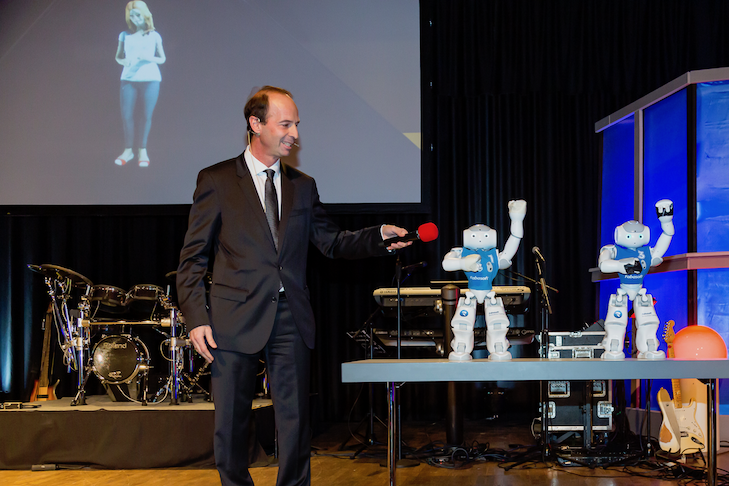
\includegraphics[scale=0.38]{img/ballDerLeondinger.png}
\end{center}
\caption{Ball der Leondinger 2019}
\label{fig:ballDerLeondinger}
\end{figure}

\begin{figure}
\begin{center}
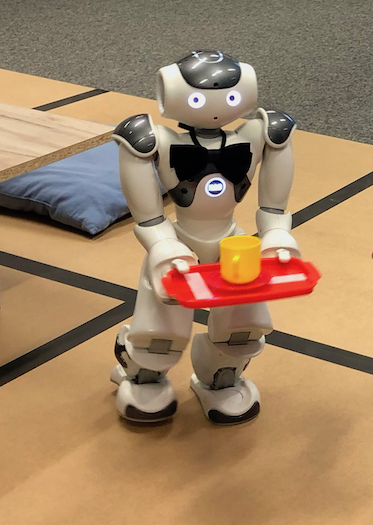
\includegraphics[scale=0.38]{img/rcjWaiter.png}
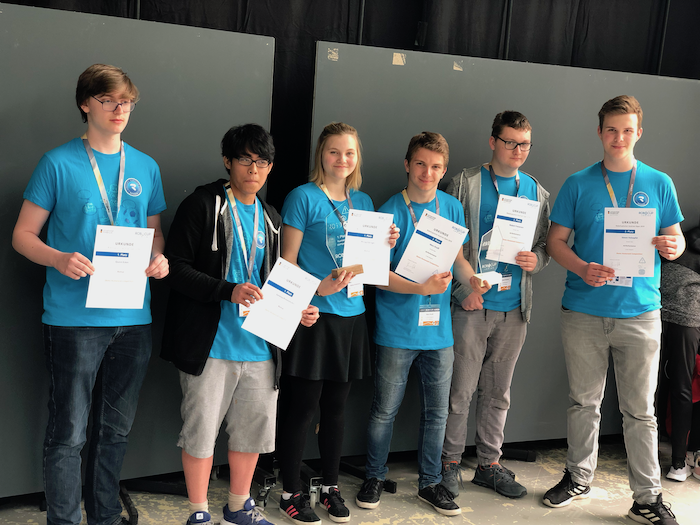
\includegraphics[scale=0.38]{img/rcjCeremony.png}
\end{center}
\caption{Demo Humanoid Challenge 2019}
\label{fig:rcjWinners}
\end{figure}

\begin{itemize}
	\item {\em Ars Electronica Festival (October 10 to 13, 2018):} The Naos were present at all five days of the Ars Electronica Festival and we showed young coders how to program humanoid robots.
	
	\item {\em Messe Jugend und Beruf (October 10 to 13, 2018):}  The Naos were present at all four days of the trade fare "Jugend und Beruf". A lot of junior students were attracted by our robots and hopefully will find their way to our school in Fall 2019.
	
	\item  {\em Ball der Leondinger (January 19, 2019):}  This dance carried the motto Leonding 2030. Our robots welcomed the guests, and guided them from the ball room entry over the wardrobes to their seats. As a highlight the Naos opened the ball together with Leonie the Avatar of the HTL Leonding (see figure~\ref{fig:ballDerLeondinger}).

	\item  {\em Schnuppertag der NMS Wartberg/Krems (January 19, 2019):}  About 20 students of the NMS Wartberg an der Krems visited the HTL Leonding and had a great time with our Naos.

	\item {\em Tag der offenen Tür at the HTL Leonding (Jan 26 and 27, 2019):}  Our Naos entertained the guests sitting at the cafeteria.
	
	\item  {\em Visit of the President of the Federal Austrian Government (January 31, 2019):}  Our Naos asked the president Wolfgang Sobotka a question concerning robots, artificial intelligence and democracy.
	
	\item {\em Austrian Open of the RoboCup Junior (Apr 25 and 26, 2019):}  Great results: Our teams (Backup and AI-Performance) won the first and the second prize in the Demo Humanoid Challenge.

	\item  {\em CoderDojo at the Didcata Digital Austria (May 24, 2019):}  Our Naos inspired some young coders at the Design Center in Linz.

	\item  {\em CoderDojo at the Diesterwegschule in Linz (Jun 26, 2019):}  Our Naos inspired some young coders at the VS 20 in Linz.

	\item  {\em Best Nao (Jun 29, 2019):}  One of our Naos presents a photobook to a bride at a wedding at Maria Enzersdorf.

	\item {\em Standard Platform League:} During this period it was possible to bring in a completely new version of the lower layers of our software, like the vision and the motion engine. We have now a much better basis for our strategy layers.
	
	\item {\em Web Site and Video:} We again took up our activities in this direction and have a prototype of a web site and a promotional video now. Both parts should be finished in the quarter 4 of 2019.
\end{itemize}

\begin{figure}
\begin{center}
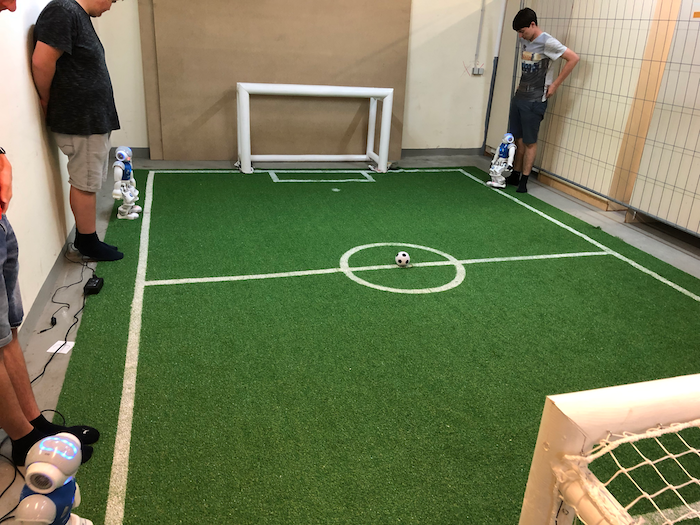
\includegraphics[scale=0.38]{img/soccerTraining.png}
\end{center}
\caption{Training of our Soccer Team}
\label{fig:soccerTraining}
\end{figure}

\subsection{Demo Humanoid Challenge}\label{sec:demoHumanoidChallenge}
After the big success at the Austrian Open 2018 it was a great experience to send again two teams to the Austrian Open 2019 in Innsbruck. This year's challenge was to implement a restaurant waiter. The program had to deal with reservations of tables, recognition of regular guests, serving drinks and food, etc.

After the first day of competition it became pretty apparent that our teams will dominate the challenge. Nevertheless both teams gave all their best and invested another night of programming to improve their software and both teams won with a tiny difference of 1.3 points whereas the third prize winning team followed with a gap of about 50 points. Figure~\ref{fig:rcjWinners} shows a typical situation at the competition and both teams at the awarding ceremony in Innsbruck.

\subsection{Standard Platform League}\label{sec:spl}
Since the achievements of the other teams at the Standard Platform League concerning their Motion Engines were dramatic we decided to partner with the Technical University Hamburg to catch up with the state of the art in this point. Compared to the software we had at the time of the last report the following improvements were done:

\begin{itemize}
	\item The walk on the 8 mm turf is now very stable and the walking speed of the Naos increased by a factor 2 to 2.5. 
	\item All software parts are now integrated and we have Naos that really can play football.
	\item A tool set to debug and optimize our software is available.
\end{itemize}
Figure~\ref{fig:soccerTraining} shows a now typical training situation.

\section{Finance}
From the 15.600 Euros we raised for this period we bought two new Naos so we have basically seven Naos available. The list of them is given in table~\ref{tab:naos}. Unfortunately we have to say that Judy, Luc and Sue are already out of maintenance, partly broken and, therefore, only of limited use to our team. So we currently may rely on a set of four Naos.

\begin{table}
\begin{center}
\begin{tabular}{|p{.3\linewidth}|p{.1\linewidth}|p{.2\linewidth}|}
\hline
\cellcolor{gray!100}\textcolor{white}{Name} & \cellcolor{gray!100}\textcolor{white}{Model} & \cellcolor{gray!100}\textcolor{white}{Year of Purchase} \\ \hline
Donald & V6 & 2018 \\ \hline
Grace & V6 & 2018 \\ \hline
Tom & V5 & 2016 \\ \hline
Anastasia & V5 & 2016 \\ \hline
Judy & V5 & 2011 \\ \hline
Luc & V5 & 2010 \\ \hline
Sue & V4 & 2009 \\ \hline
\end{tabular}
\end{center}
\caption{Currently available Naos}
\label{tab:naos}
\end{table}

\section{Planned Activities for 2019/20}

\begin{itemize}
	\item {\em Public Events:}  As last year we plan to have at least 10 appearances with our Naos.
	
	\item {\em New Nao:} With another Robot, we will get a team of 5 robots which can be used without limitations. This brings us into a position to provide a full soccer team for the Standard Platform League. Nevertheless it will be necessary to increase the number of robots by another two or three during the next years in order to have a few substitutes available.
	
	\item {\em RoboCup Junior Austrian Open (April 24 and 25, 2020):} Besides the goal to win the Demo Humanoid Challenge also next year, we want to bring in more teams from other schools to make the challenge more exciting. This shall be a good basis to bring this challenge to a better attention at the RoboCup International.
	
	\item {\em RoboCup German Open:} Since we gained big improvements in our soccer software we dare to approach the Standard Platform League at the German Open 2020 in Magdeburg.
	
	\item {\em Marketing Activities:} As mentioned we shifted parts of our activities so we still want to set up a web site and a promotional video in order to make our activities better visible to a wider audience.
\end{itemize}

\section{Acknowledgements}
This project would not be possible without the kind support of several persons and organizations. We would like to express our gratitude to:

\begin{itemize}
	\item \emph{Absolventenverein der HTL Leonding (AbsLeo):} The AbsLeo accompanies this project since 2009. It budgeted the initial hardware which allowed us to get first experience with the Naos, renewed our hardware in Fall 2016, and contributed to the new Naos bought in Fall 2018. Although it was clear that the whole journey will be a long one we could rely on their constant support. This enabled us to continue our ambitions towards participating the RoboCup World Championships.
	
	\item \emph{Management of the HTL Leonding:} Every project needs the great support from its embedding organization. All the smaller and larger organizational issues we are facing can be solved by means of the friendly support of our school. This is enabled by our head master and the two heads of departments. We are very happy to know that we can rely on them.
	
	\item \emph{Thomas Himmelbauer:} Despite his tough schedule as our school's IT manager he is a great technical supporter of our project. Especially if it comes to support our team in the small but important technical questions, from providing power distributions to software tools, he is always a great help.
\end{itemize}

\end{document}  